\documentclass{beamer}
 
\usepackage[utf8]{inputenc}
\usepackage{minted}
\usepackage{tcolorbox}
\usepackage{etoolbox}
\BeforeBeginEnvironment{minted}{\begin{tcolorbox}}
\AfterEndEnvironment{minted}{\end{tcolorbox}}

\usetheme{Madrid}
\usecolortheme{beaver}
 
\title{An Introduction to \LaTeX}
\author{ACM}
\institute{New York University}
\date{2019}
 
\begin{document}

 
\frame{\titlepage}
 

\begin{frame}
\frametitle{Why the f*** does this exist?}
Most of us begin our word processing journey with huble intentions

\[
\text{\textbf{Get the thing typed!}}
\]

So why bother with \LaTeX\@?

\end{frame}


\begin{frame}
\frametitle{Why the f*** does this exist?}

\begin{enumerate}

    \item It's beautiful.

        \begin{itemize}
            \item \textit{Especially} for math.
            \item Try and find a paper on Arxiv not written in \LaTeX.
        \end{itemize}

    \item It was created by scientists, for scientists.

        \begin{itemize}
            \item Large and active community.
            \item Online support is readily found.
        \end{itemize}

    \item It's powerful; extremely rich package community.

\end{enumerate}

\end{frame}

\begin{frame}
    \frametitle{Who's it for?}
    \begin{enumerate}
        \item<1-> Created by scientists, for scientists.
            \begin{itemize}
                \item Journal articles and theses, with or without complex
                    math notation.
                \item The technical publishing industry.
                \item Your professors when cooking up problem sets to torture
                    you with.
            \end{itemize}
        \item<2-> Not a word processor.
            \begin{itemize}
                \item No spell check\footnote{Technically untrue, see
                        ispell}.
                \item No complete control over formatting.
            \end{itemize}
        \item<3-> ``You take care of writing, and we'll take care of
            presentation.``
    \end{enumerate}
\end{frame}

\begin{frame}
    \frametitle{How does this work?}
    \begin{enumerate}
        \item You specify the input in a source file.
            \begin{itemize}
                \item Vi/Vim, Emacs, Sublime, \dots
                \item TeXMaker, TeXStudio, \dots
            \end{itemize}
        \item LaTeX processes the content and decides how best to typeset it.
    \end{enumerate}
    \vspace{0.5cm}
    \begin{framed}
        \mintinline{latex}{I have a test \textbf{tomorrow}, but here I
            am \dots}
    \end{framed}
    \[
        \Downarrow
    \]
    \begin{framed}
        I have a test \textbf{tomorrow}, but here I am \dots
    \end{framed}
\end{frame}

\begin{frame}[fragile]
\frametitle{Some Examples\dots}

\begin{minted}{latex}
\begin{enumerate}
\item \textit{Very} important first thing.
\item \textbf{Extremely} important second thing.
\item \underline{Ultra} important third thing.
\end{enumerate}
\end{minted}

\[ \Downarrow \]

\begin{enumerate}
\item \textit{Very} important first thing.
\item \textbf{Extremely} important second thing.
\item \underline{Ultra} important third thing.
\end{enumerate}

\end{frame}
 
\begin{frame}[fragile]
\frametitle{Some Examples\dots}

\begin{minted}{latex}
\begin{figure}
    \centering
    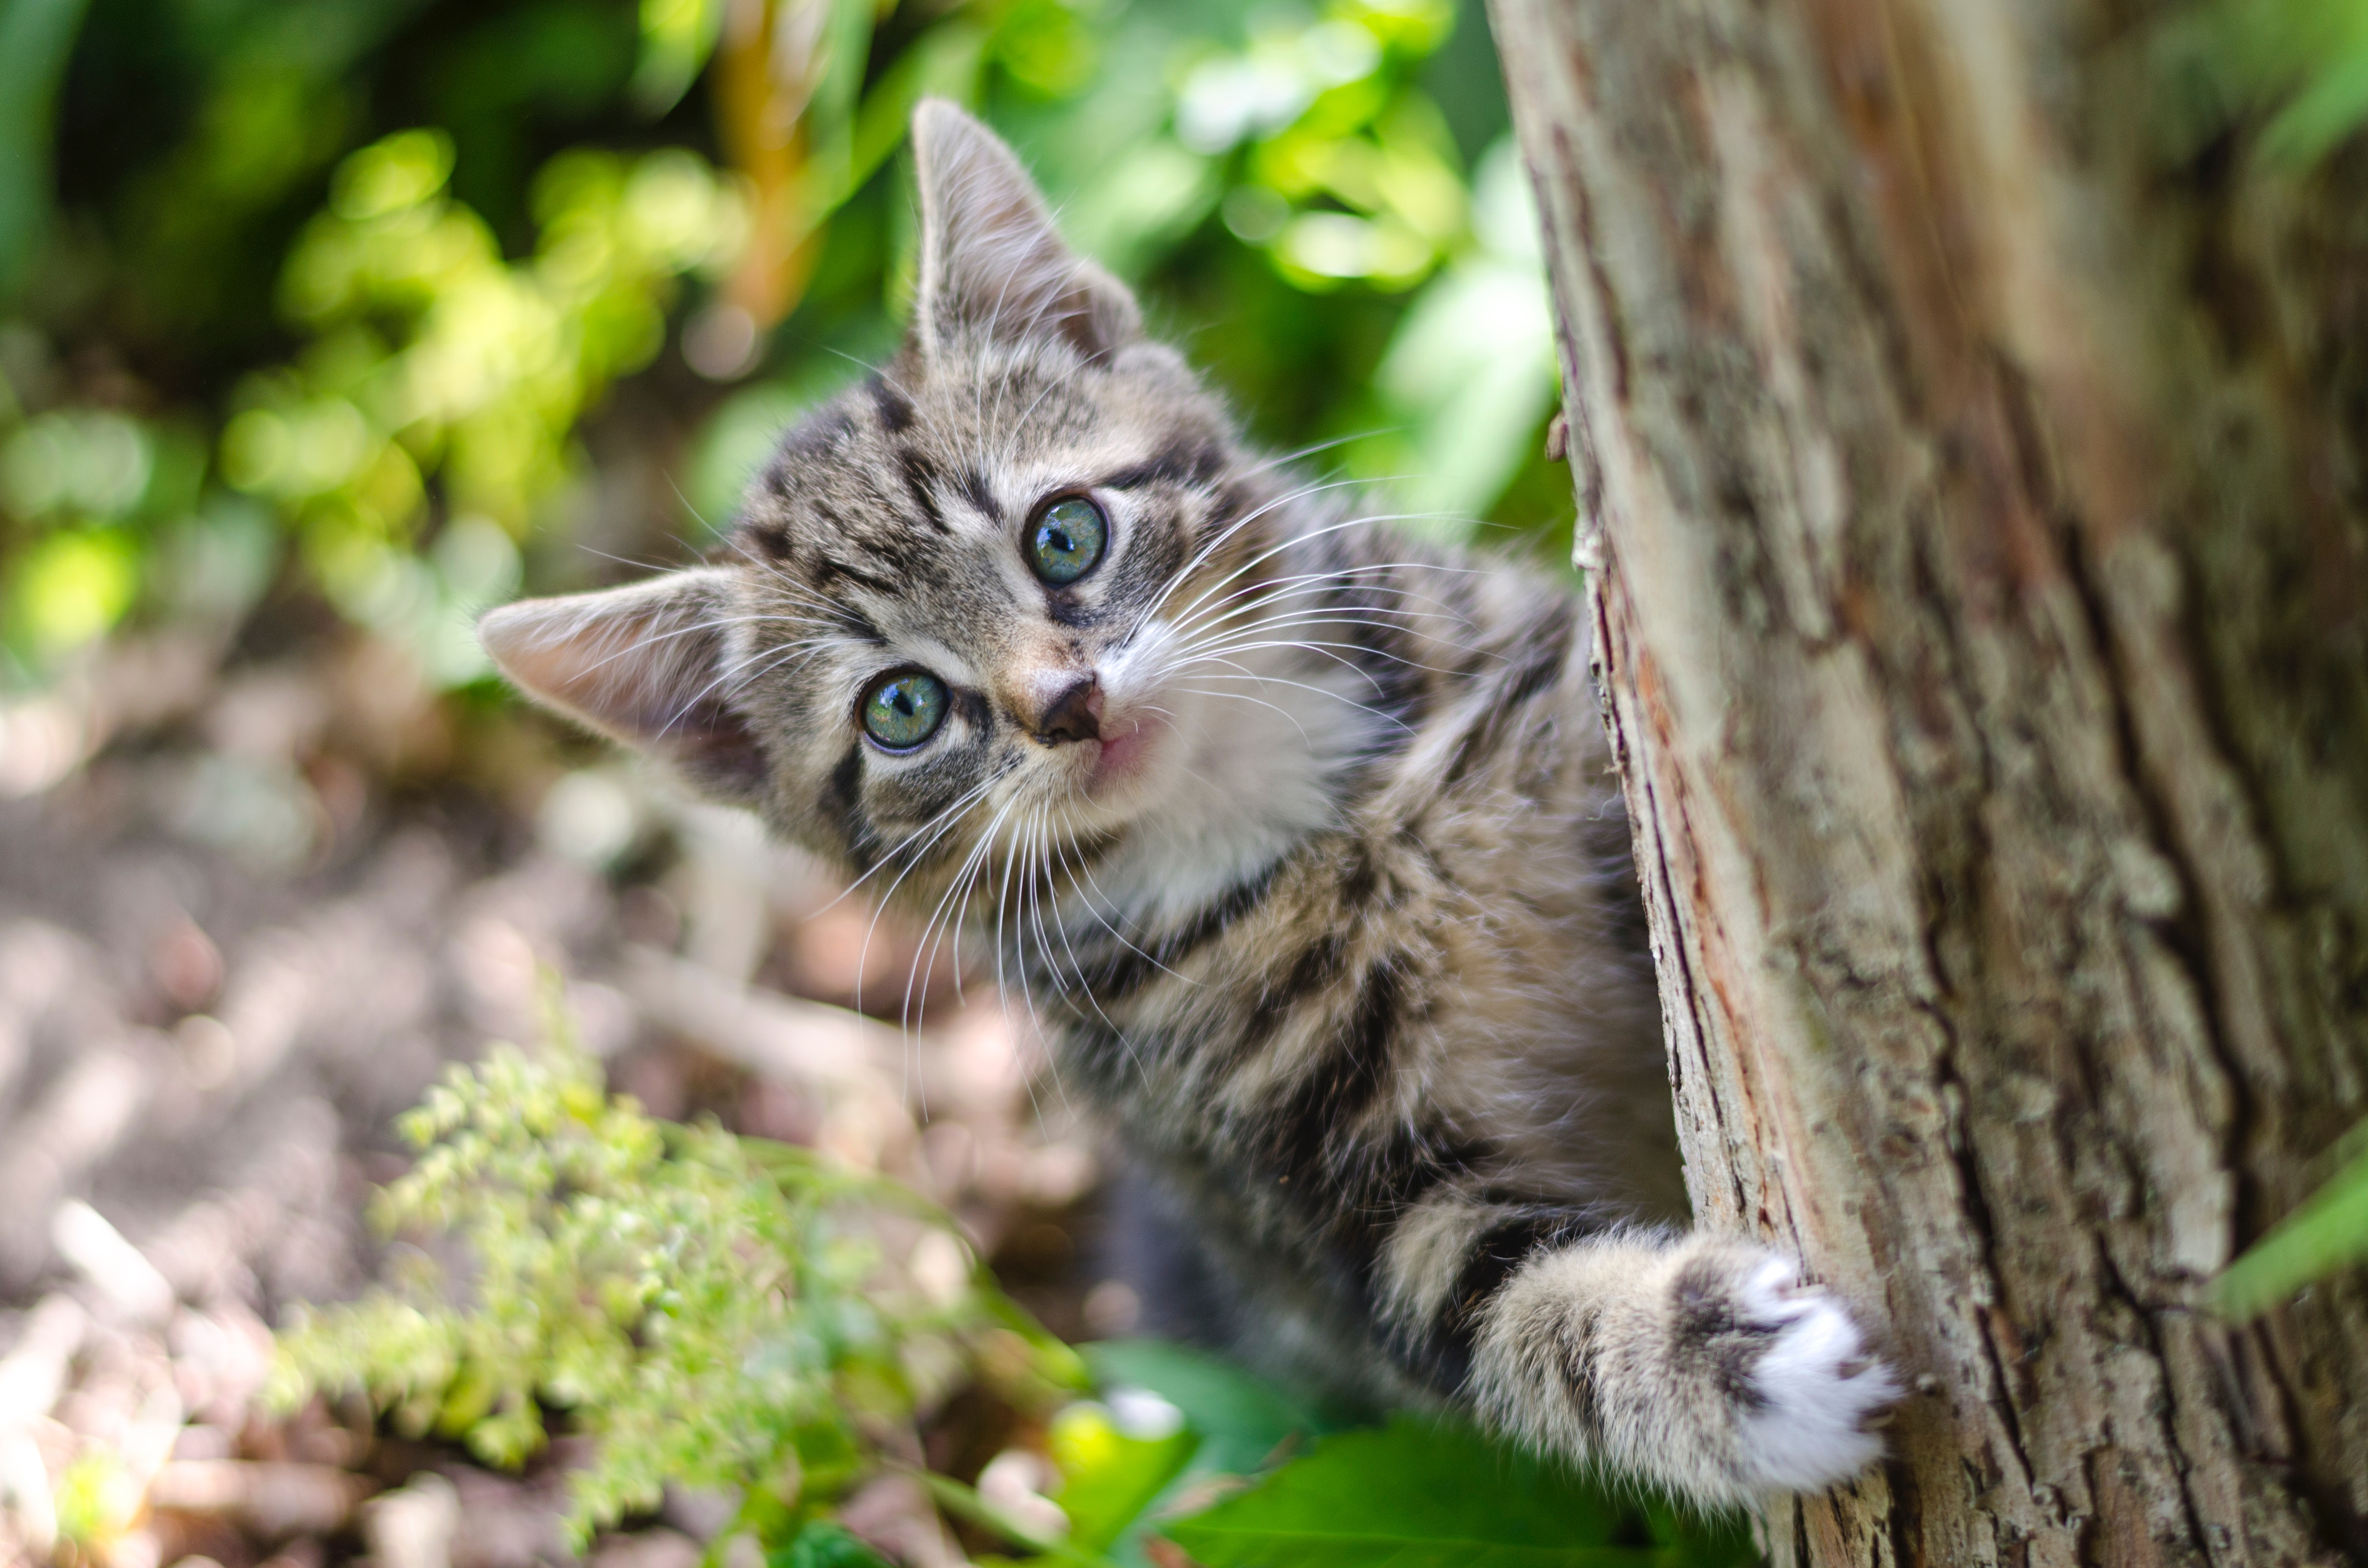
\includegraphics{./cat.jpg}
\end{figure}
\end{minted}

\[ \Downarrow \]

\begin{figure}
    \centering
    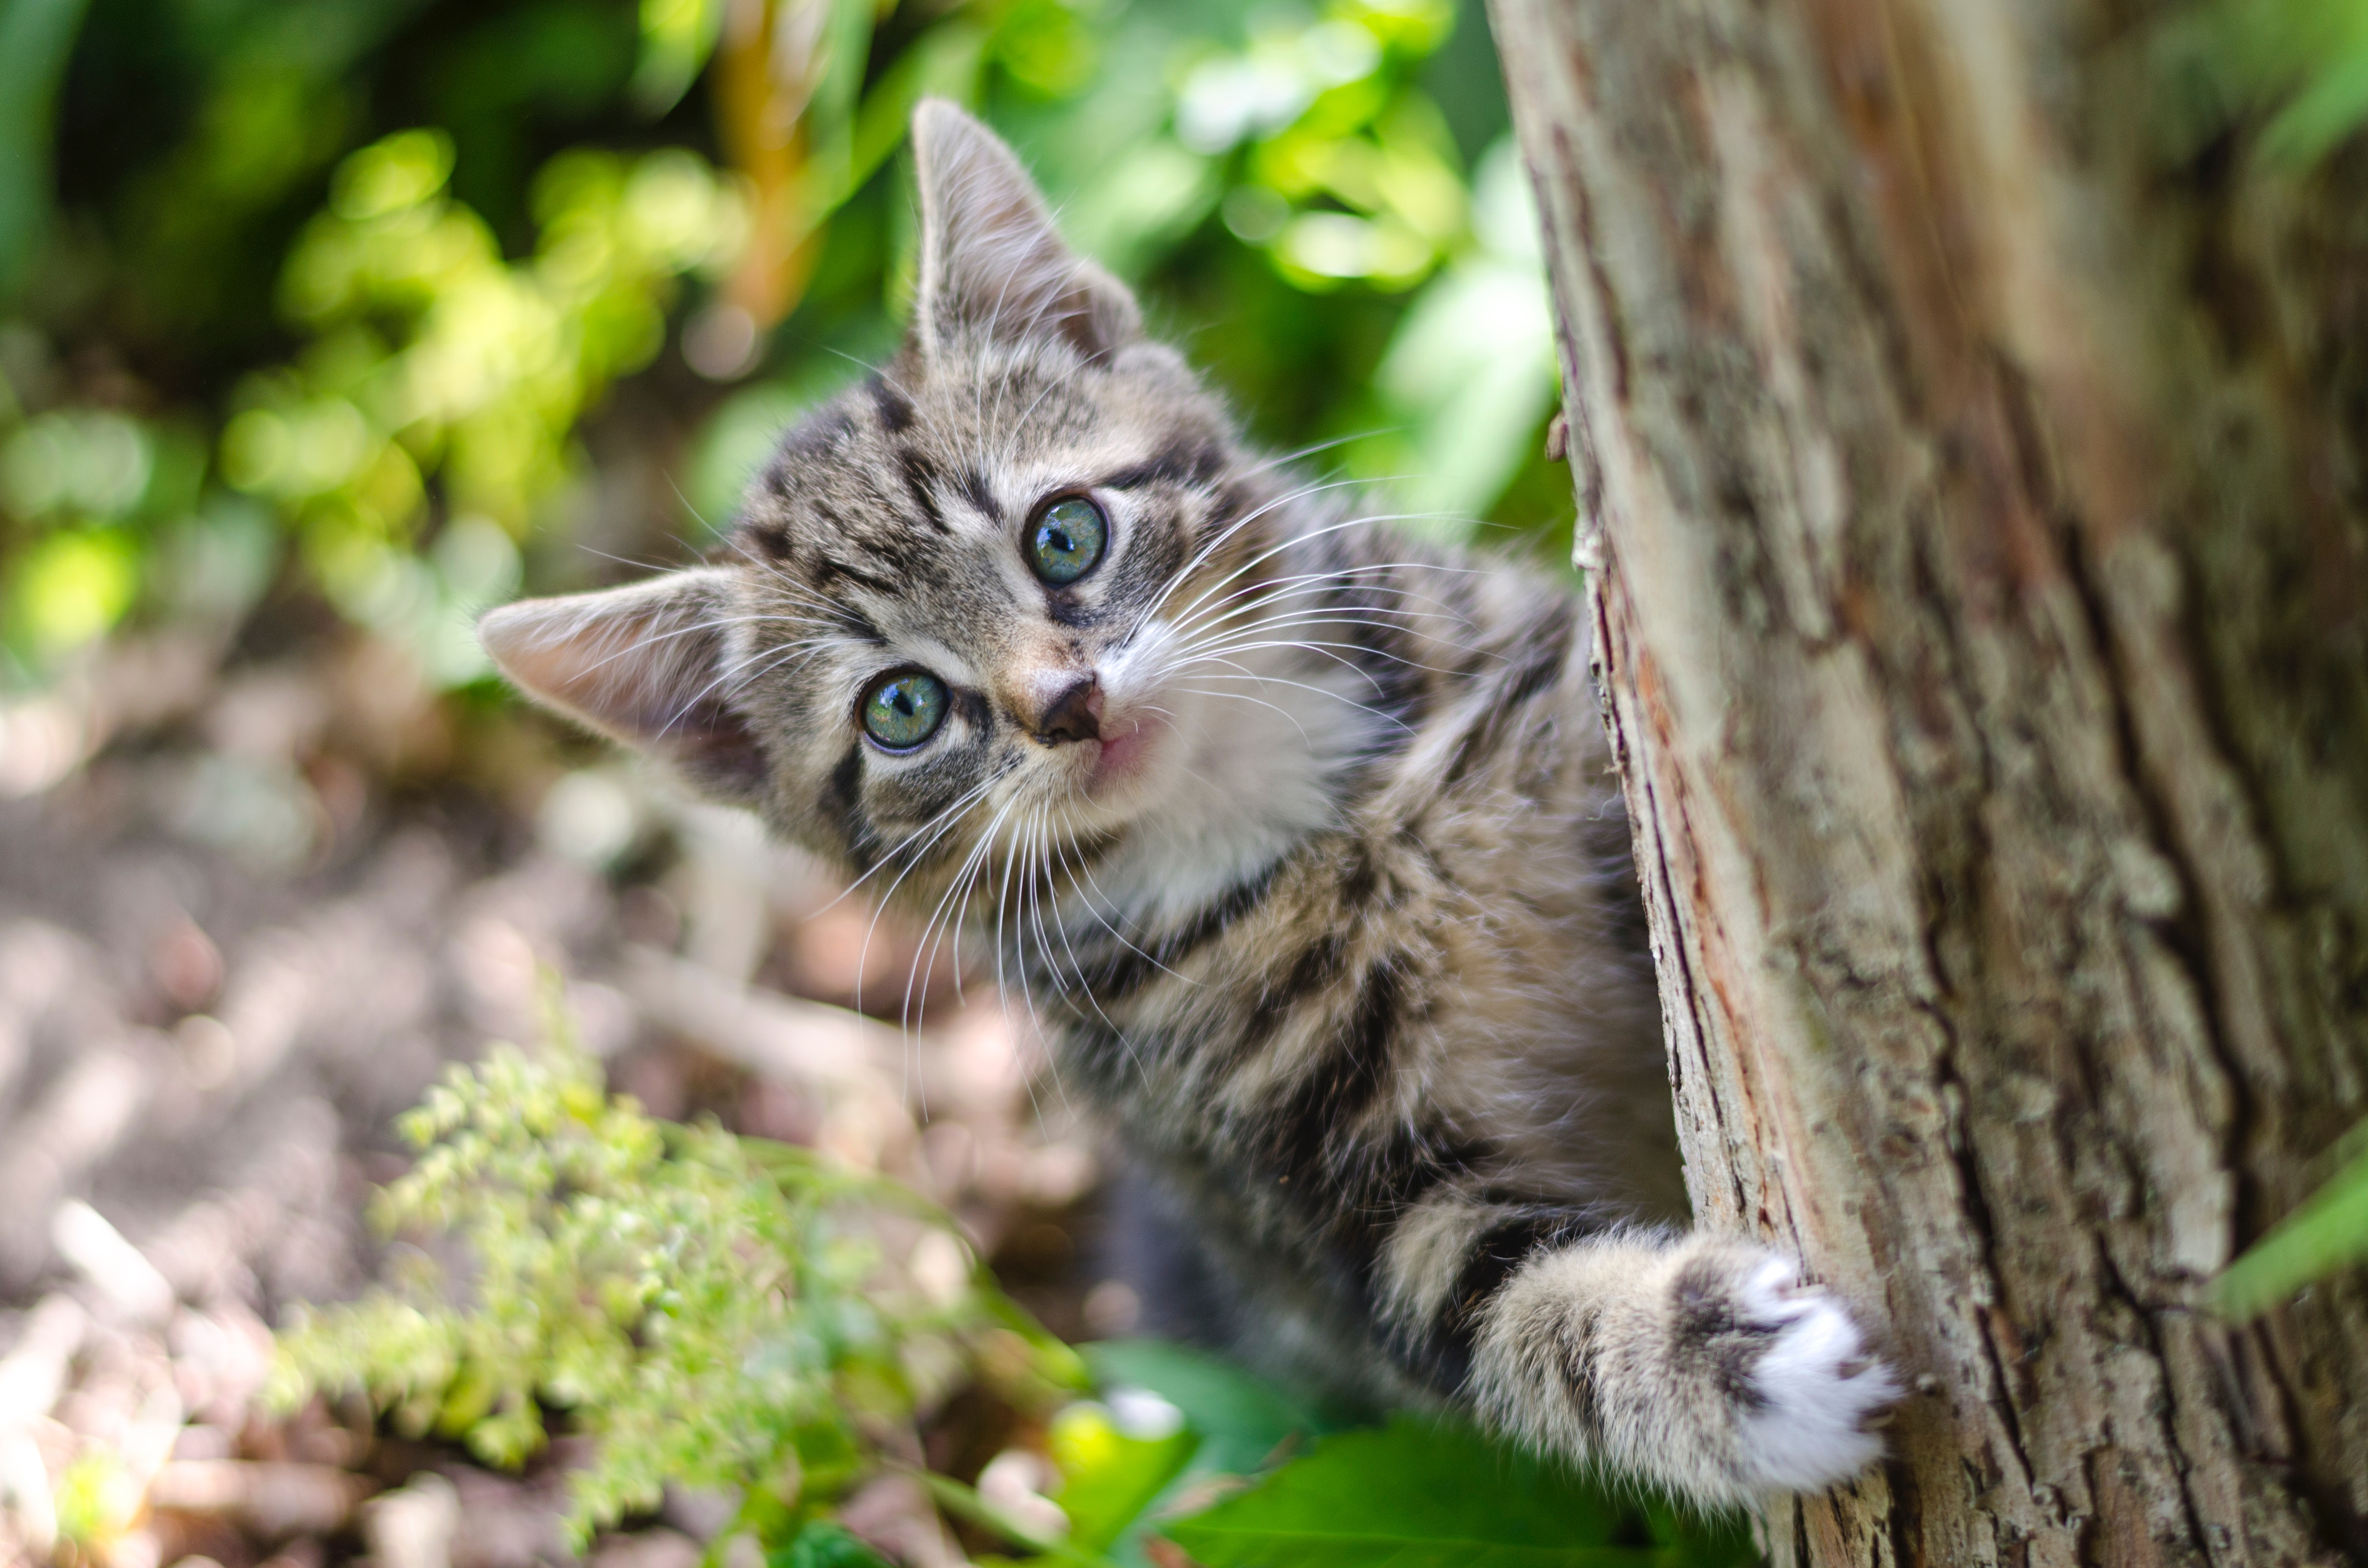
\includegraphics[width=.4\textwidth]{./cat.jpg}
\end{figure}

\end{frame}

\begin{frame}[fragile]
\frametitle{Some Examples\dots}

\begin{minted}{latex}
$\forall \varepsilon > 0, \exists \delta > 0$ such that 
if $d(x, y) < \delta \implies d(f(x), f(y)) < 
\varepsilon$.
\end{minted}

\[ \Downarrow \]

\begin{framed}
$\forall \varepsilon > 0, \exists \delta > 0$ such that 
if $d(x, y) < \delta \implies d(f(x), f(y)) < 
\varepsilon$.
\end{framed}

\end{frame}

\begin{frame}[fragile]
\frametitle{Shift in perspective}

If you're coming from a WYSISYG editor, the above may look complicated and
annoying.

\begin{enumerate}
\item<1-> You're right; kinda. There's a learning curve for the syntax.
\item<2-> Describe ``What it is'', not ``How it looks''.
\item<3-> Let \LaTeX\@ and it's packages do the rest.
\end{enumerate}

\end{frame}

\begin{frame}[fragile]
\frametitle{Packages: Infinite Power}

Packages are varied, powerful, and sometimes hilarious.

\begin{enumerate}
    \item<1-> Beamer. Slideshow documentclass, what this is written on!
    \item<2-> Minted, Code highlighter.
    \item<3-> amsmath, amsthm, etc. Amazing extended math symbols from AMS.
    \item<4-> Fun packages:
        \begin{enumerate}
            \item Coffee Stains.
            \item avremu. Technically \LaTeX\@ is turing complete so\dots
        \end{enumerate}
\end{enumerate}

\end{frame}

\begin{frame}[fragile]
\frametitle{Learning \LaTeX\@}

\begin{enumerate}
    \item<1-> Not hard, but slow. You must build your vocabulary!
    \item<2-> Start \LaTeX'ing!
\end{enumerate}

\end{frame}

\begin{frame}[fragile]
\frametitle{Beginnings}

\begin{minted}{latex}
\documentclass{article}
\begin{document}
Salve, munde! %minted coloring latex in latex
\end{document}
\end{minted}

\end{frame}

\begin{frame}[fragile]
\frametitle{Beginnings}

\begin{minted}{latex}
\documentclass{article}
\begin{document}
Salve, munde! %minted coloring latex in latex
\end{document}
\end{minted}

Ok \dots, now we have code. How do we turn this into something usable?

\end{frame}

\begin{frame}[fragile]
\frametitle{Practical Demo: Introduction of Enviornments}

\begin{enumerate}
\item GUI: Overleaf
\item CLI: pdflatex and pandoc+markdown.
\end{enumerate}

\end{frame}

\end{document}
